\chapter{分治算法之平面最近点对问题}

\begin{introduction}
\item 平面最近点对问题定义
\item 分治算法设计及伪代码
\item 分治算法正确性证明及复杂度分析
\end{introduction}

\section{平面最近点对问题定义}
给定二维平面上的$n(n \ge 2)$个不同的点$p$组成点集$P = \{p_i \big| 1\le i \le n\}$,
设计算法寻找欧式距离最近的点对$(A,B)$。
\begin{figure}[htb]
    \centering
    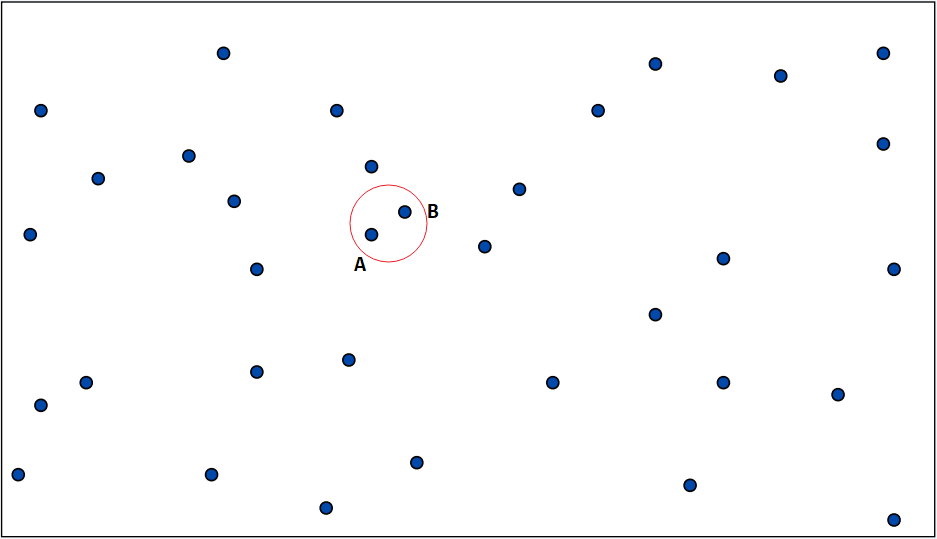
\includegraphics[scale=0.5]{Ln9.image/NearestPointsDef.png}
    \caption{问题定义图例}\label{fig1}
\end{figure}

如上图\autoref{fig1}中点对$(A,B)$即为问题的答案。

\section{分治算法设计及伪代码}
对于这样一个问题,我们很直接地可以使用BF (Brute Force)算法进行暴力求解,
即二重循环计算所有点之间的距离,从而获得最小距离,显然该算法的时间复杂度为
$O(n^2)$。那么有没有更快的算法呢?本章我们使用经典的算法思想——分治,
设计一个$O(n\log n)$的算法。

\subsection{分治问题}
遵循分治思想,我们首先要考虑如何分治问题使得问题规模约减。

我们使用X坐标作为第一关键字、Y坐标作为第二关键字,对点集$P$进行排序,
并以点$p_{\lfloor\frac{n}{2}\rfloor}$作为分治点,获得如下两个点集:
\begin{equation*}
    P_1 = \{p_i\ \big|\ 1 \le i \le \lfloor\frac{n}{2}\rfloor \}
\end{equation*}
\begin{equation*}
    P_2 = \{p_i\ \big|\ \lfloor\frac{n}{2}\rfloor < i \le n\}
\end{equation*}
这样就将当前问题约减为两个规模为$\lfloor\frac{n}{2}\rfloor$的子问题。
分治过程如\autoref{fig2}中所示。

\begin{figure}[htb]
    \centering
    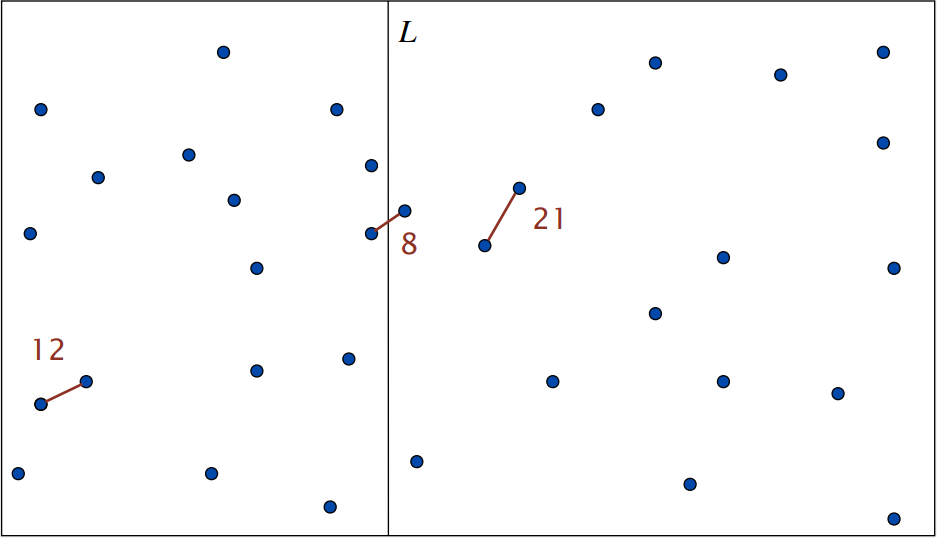
\includegraphics[scale=0.5]{Ln9.image/NearestPointsDivide.png}
    \caption{分治过程图例}\label{fig2}
\end{figure}

如此递归下去,我们可以求得两个点集相对应的最近点对距离$\delta_1, \delta_2$,取其中较小值
记为$\delta = \min \{ \delta_1 , \delta_2 \}$。


\subsection{合并结果}

接着,我们需要考虑如何合并子问题的解。

上述的$\delta$一定是正确的合并结果嘛?显然不是,我们并没有考虑,一端在$P_1$,
一端在$P_2$的线段。因此,在合并阶段,我们要将这种情况考虑在内。

这里,我们将所有横坐标与分治点$p_{\lfloor\frac{n}{2}\rfloor}$的横坐标
$x_{\lfloor\frac{n}{2}\rfloor}$差值小于$\delta$的点组成集合$B$,即
\begin{equation*}
    B = \{p_i\ \big|\ 
        \left|x_i - x_{\lfloor\frac{n}{2}\rfloor}\right| \le \delta ,\
        1 \le i \le n\}
\end{equation*}   
因为只有$B$集合中的点之间的距离才有可能小于$\delta$。
$B$集合如下图\autoref{fig3}中阴影部分所示:
\begin{figure}[htb]
    \centering
    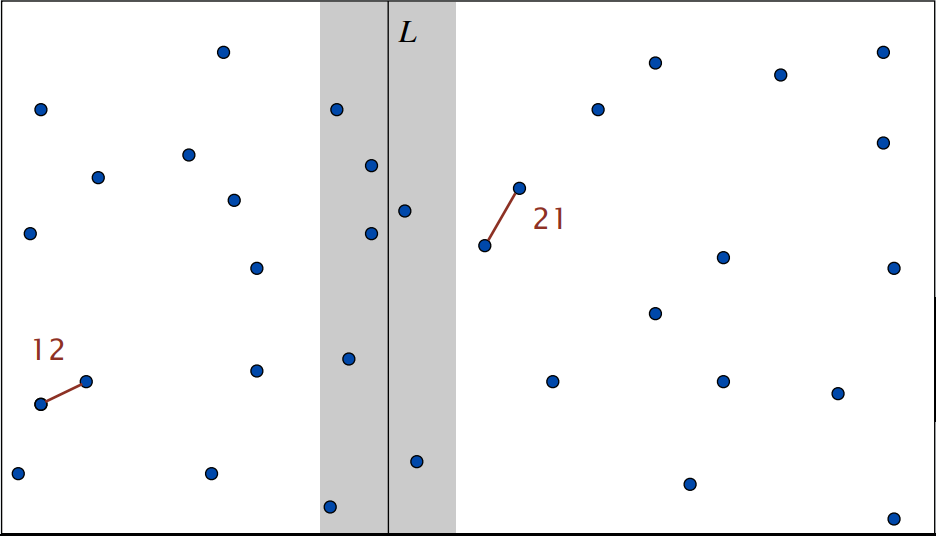
\includegraphics[scale=0.5]{Ln9.image/NearestPointsMerge.png}
    \caption{合并过程图例}\label{fig3}
\end{figure}

进一步,我们的目标是检验在$B$集合中是否存在距离比$\delta$更近的点对,以此更新当前问题的解
。因此,对于每个$p_i = (x_i, y_i) \in B$遍历所有在其之下竖直距离不超过$\delta$的点,
即遍历集合
\begin{equation*}
    C(p_i) = \{ p_j\ \big|\ y_i - \delta \le y_j \le y_i, p_j \in B \}
\end{equation*}
为了方便遍历,这里需要对$B$集合中的点,以Y坐标为第一关键字,X坐标为第二关键字,进行排序。

至此,我们完成了父问题的分治与子问题的合并。

\subsection{伪代码}
\begin{algorithm}
    \DontPrintSemicolon{}
    \KwData{Point Set $P = \{p_i\ \big|\ 1 \le i\le n, p_i = (x_i, y_i)\}$}
    \KwResult{the nearest pair $(A, B)$}
\Begin{
    Sort points in $P$ by x-coordinate in descending order\;
    $m \leftarrow \lfloor \frac{n}{2} \rfloor$\;
    $\delta_1 \leftarrow \text{Nearest-Pair}(P[1,\ \ldots,\ m])$\;
    $\delta_2 \leftarrow \text{Nearest-Pair}(P[m + 1,\ \ldots ,\ n])$\;
    $\delta \leftarrow \min \{ \delta_1, \delta_2 \}$\;
    $B \leftarrow \{ \}$\;
    \ForEach{$p_i\in P$}{
        \If{$\left| x_i - x_m\right| \le \delta$}{
            $\text{add } p_i \text{ to } B$
        }
    }
    Sort points in $B$ by y-coordinate in descending order\;
    \For{$i \leftarrow 1 $ \KwTo$|B|$}{
        \For{$j \leftarrow i + 1$ \KwTo$|B|$} {
            \If{$\left| y_i - y_j \right| \le \delta$}{
                $\delta \leftarrow \min \{ \delta ,\ \text{Euclidean-Distance}(p_i,\ p_j) \}$
            }
        }
    }
    Return $\delta$
}
\caption{Nearest-Pair\label{NPP}}
\end{algorithm}

\section{分治算法正确性证明与复杂度分析}
